% =====================================================================
%  MSc dissertation — Implementation Progress Report (illustrated, code-grounded walkthrough)
%  Predicting the Zero-Shot Transfer of a Promptable Video Tracker (SA-FARI / SAM 3)
%  Build:  report/build.sh report/progress   (Tectonic + Ghostscript-normalise)
% =====================================================================
\documentclass[11pt,a4paper]{article}

\usepackage[a4paper,margin=2.3cm]{geometry}
\usepackage{iftex}
\ifPDFTeX
  \usepackage[T1]{fontenc}
  \usepackage[utf8]{inputenc}
  \IfFileExists{lmodern.sty}{\usepackage{lmodern}\usepackage{microtype}}{}
\else
  \usepackage{fontspec}
  \IfFileExists{microtype.sty}{\usepackage{microtype}}{}
\fi
\usepackage{amsmath,amssymb}
\usepackage{booktabs}
\usepackage{enumitem}
\usepackage{caption}
\usepackage[dvipsnames]{xcolor}
\usepackage{tikz}
\usetikzlibrary{positioning,arrows.meta,calc}
\usepackage{pgfplots}
\pgfplotsset{compat=1.18}
\usepackage{listings}
\usepackage[colorlinks=true,linkcolor=NavyBlue,urlcolor=NavyBlue]{hyperref}

\definecolor{navy}{RGB}{30,64,124}
\definecolor{forest}{RGB}{34,120,60}
\definecolor{burnt}{RGB}{214,104,26}
\definecolor{plum}{RGB}{140,55,135}
\newcommand{\done}{{\color{forest}\textbf{done}}}
\newcommand{\built}{{\color{navy}\textbf{built}}}
\newcommand{\todo}{{\color{burnt}\textbf{next}}}
\newcommand{\code}[1]{\texttt{#1}}
\setlist{nosep,leftmargin=1.4em}
\captionsetup{font=small,labelfont=bf}

% shared TikZ flow-box styles
\tikzset{
  box/.style={draw,rounded corners,align=center,font=\footnotesize,inner sep=4pt,minimum height=0.9cm},
  data/.style={box,fill=black!5},
  work/.style={box,fill=navy!12},
  resbox/.style={box,fill=burnt!16},
  flow/.style={-{Latex[length=2mm]},thick},
}

% ---- code listing style (Python) ----
\definecolor{codebg}{RGB}{247,247,251}
\definecolor{codekw}{RGB}{30,64,124}
\definecolor{codecm}{RGB}{110,122,134}
\definecolor{codestr}{RGB}{34,120,60}
\lstdefinestyle{py}{
  language=Python,
  basicstyle=\ttfamily\scriptsize,
  keywordstyle=\color{codekw}\bfseries,
  commentstyle=\color{codecm}\itshape,
  stringstyle=\color{codestr},
  backgroundcolor=\color{codebg},
  frame=leftline,
  framerule=1.4pt,
  rulecolor=\color{navy!45},
  numbers=none,
  showstringspaces=false,
  breaklines=true,
  keepspaces=true,
  columns=fullflexible,
  xleftmargin=0.9em,
  aboveskip=0.4em,belowskip=0.7em,
}
\lstset{style=py}
% filename banner printed just above a listing
\newcommand{\srcfile}[1]{\smallskip\noindent{\footnotesize\color{navy}\ttfamily\textbf{#1}}\par\nobreak\vspace{-0.15em}}
% green takeaway callout
\newcommand{\takeaway}[1]{\smallskip\noindent%
  \colorbox{forest!8}{\parbox{\dimexpr\linewidth-2\fboxsep\relax}{%
  \small{\color{forest}\textbf{Takeaway.}}\ #1}}\smallskip}

\title{\vspace{-1.6em}\textbf{Implementation Progress Report}\\[3pt]
\large How each step works, in plain words and in the code\\[1pt]
\normalsize Predicting the Zero-Shot Transfer of a Promptable Video Tracker (SAM\,3 on SA-FARI)}
\author{Kostiantyn Boiar \,\textbullet\, Supervisor: Dr Marwa Mahmoud\\
\normalsize School of Computing Science, University of Glasgow}
\date{\today}

\begin{document}
\maketitle
\vspace{-1.0em}

\noindent
This report walks through \emph{everything built so far}, one step at a time, and for each step it answers
three questions: \textbf{what is the point} of it, \textbf{what does the code actually look like}, and
\textbf{what is that code doing}, line by line, in plain words. The one-line goal of the whole project:
given a new animal in a new place, \textbf{predict how well SAM\,3 will track it \emph{before} we run it},
and explain \emph{why} --- separately for \textbf{finding} the animal (\code{pDetA}) and \textbf{following}
it (\code{pAssA}).

\smallskip\noindent
\textit{How to read each step:} a \textbf{``The point''} paragraph (why it exists) $\rightarrow$ a real
slice of the \textbf{code} on disk $\rightarrow$ an \textbf{``In the code''} plain walk-through of that
slice $\rightarrow$ a green \textbf{Takeaway}. Diagrams and real-data charts appear where a picture explains
the mechanism faster than words.

\begin{figure}[h]
\centering
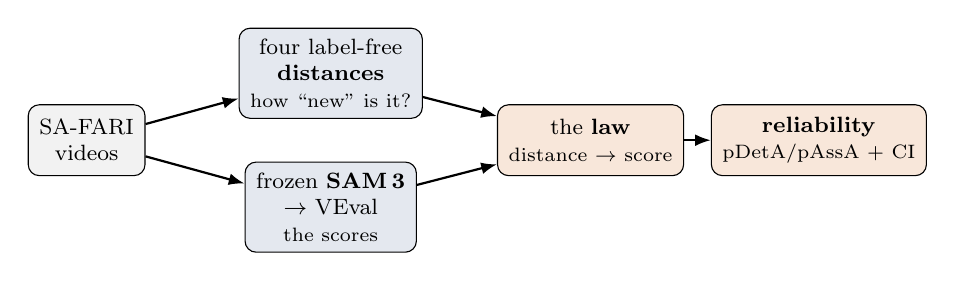
\begin{tikzpicture}
  \node[data] (saf) at (0,0) {SA-FARI\\videos};
  \node[work] (dist) at (3.1,0.85) {four label-free\\\textbf{distances}\\{\scriptsize how ``new'' is it?}};
  \node[work] (sam) at (3.1,-0.85) {frozen \textbf{SAM\,3}\\$\to$ VEval\\{\scriptsize the scores}};
  \node[resbox] (law) at (6.4,0) {the \textbf{law}\\{\scriptsize distance $\to$ score}};
  \node[resbox] (rel) at (9.3,0) {\textbf{reliability}\\{\scriptsize pDetA/pAssA $+$ CI}};
  \draw[flow] (saf) -- (dist);
  \draw[flow] (saf) -- (sam);
  \draw[flow] (dist) -- (law);
  \draw[flow] (sam) -- (law);
  \draw[flow] (law) -- (rel);
\end{tikzpicture}
\caption{The whole system in one picture. The \textbf{distances} (top) are the inputs $X$; the frozen
\textbf{SAM\,3} scores (bottom) are the outputs $Y$; we fit a small \textbf{law} $X\!\to\!Y$ and turn it into
a \textbf{reliability} estimate. The distance side is complete; the score side is built and awaiting a GPU run.}
\end{figure}

\vspace{-0.4em}
\begin{center}\small
\begin{tabular}{@{}lp{11.4cm}@{}}
\toprule
\textbf{Where we are} & \\
\midrule
\done   & data acquisition; dataset/schema reader; the two experiments $+$ frozen reference; all four
          label-free distances (taxonomic, temporal, visual, environment); the shared embedding pipeline;
          the leakage firewall $+$ tests.\\
\built  & SAM\,3 inference harness $+$ VEval scoring $+$ per-cell aggregation (run on Colab; weights access
          confirmed).\\
\todo   & SAM\,3 familiarity proxy; feature-table assembly; fit the law, cross-validation, reliability tool.\\
\bottomrule
\end{tabular}
\end{center}

% =====================================================================
\section{Step 1a --- Getting the data onto disk}

\paragraph{The point.}
Before we can measure anything, two things have to be on disk: the SA-FARI \emph{annotation files} (the
ground-truth boxes, masks and taxonomy) and the actual \emph{video frames} to run the tracker on. They live
in two different places with two different access rules --- the annotations are gated behind a Hugging Face
license click, and the frames sit in a public Google Cloud bucket. \code{src/acquire.py} is the single
entry point that pulls both. It quietly works around a token quirk and never re-downloads anything already
fetched, so a download can be stopped and restarted safely.

\srcfile{src/acquire.py}
\begin{lstlisting}[style=py]
def _frame_uri(self, split: str, file_name: str) -> str:
    """Full bucket URI for one ``file_names`` entry under the split's frame root."""
    base = self.config.data.frames_gcs_dir.format(split=split)
    return f"{self.bucket}/{base}/{file_name}"

def fetch(self, file_names: list[str], split: str) -> int:
    # ...
    if not self.fs.exists(self._frame_uri(split, file_names[0])):
        raise FileNotFoundError(
            f"cannot locate {file_names[0]!r} at {self._frame_uri(split, file_names[0])}"
        )
    dest_root = self.config.paths.data_root / self.config.data.frames_subdir
    pulled = 0
    for name in file_names:
        dest = dest_root / name
        if dest.exists():
            continue
        dest.parent.mkdir(parents=True, exist_ok=True)
        self.fs.get_file(self._frame_uri(split, name), str(dest))
        pulled += 1
    return pulled
\end{lstlisting}

\paragraph{In the code.}
Every frame lives at a predictable web address inside Google's public bucket. \code{\_frame\_uri} builds
that address: it takes a template and fills in whether we want the \emph{train} or \emph{test} set
(\code{.format(split=split)}), then glues on the bucket name and the frame's relative path (something like
\code{videoABC/frame\_0007.jpg}) to produce one full location string. \code{fetch} then does the actual
downloading, and it does three careful things. First, a \textbf{fail-fast check}: it asks the cloud
filesystem ``does the very first frame actually exist at this address?'' --- if not, it stops immediately
with a clear error, because that almost always means we asked for the wrong split, and every later download
would fail too. Second, the \textbf{skip-existing loop}: for each frame it computes where the file should
land locally (\code{dest}), and if that file is already there it simply \code{continue}s past it --- so
re-running never repeats finished work, which makes the whole pull \emph{resumable}. Third, for the frames
that are genuinely missing, it creates the folder, copies the file down (\code{get\_file}) and bumps a
counter, returning how many were newly fetched so the caller reports real progress. Separately, at the top
of the file, \code{HF\_HUB\_DISABLE\_XET = True} is a workaround: the annotation download goes through
Hugging Face, whose newer ``Xet'' transfer backend rejects fine-grained access tokens with a 403, so this
forces the plain, reliable HTTPS path instead.

\takeaway{A resumable, split-aware downloader that lands both the gated annotations and the public frames
exactly where the pipeline expects, and fails loudly on the one mistake --- the wrong split --- that would
otherwise waste a whole run.}

% =====================================================================
\section{Step 1b --- Reading the dataset (the schema)}

\paragraph{The point.}
SA-FARI ships as one big YTVIS-style JSON per split, where species names, their 7-level taxonomy, the
(video, prompt) probes, and the per-frame masks all live in \emph{separate lists linked only by numeric
ids} (Fig.~\ref{fig:schema}). \code{src/dataset.py} turns each raw probe into one clean, typed
\code{VideoRecord}: it resolves the species from its numeric \code{category\_id}, flags probes where the
queried animal is absent (\emph{hard negatives}), and exposes a NaN-safe taxonomy lookup --- so the rest of
the pipeline works with meaningful objects instead of hunting through nested JSON. It is the single trusted
place that defines what a ``probe'' is for the whole study.

\srcfile{src/dataset.py}
\begin{lstlisting}[style=py]
def records(self) -> list[VideoRecord]:
    """Return every (video, prompt) probe in the split (hard negatives included by default)."""
    data = self._load()
    videos = {v["id"]: v for v in data["videos"]}
    records: list[VideoRecord] = []
    pairs = data.get("video_np_pairs")
    if pairs:
        for pair in pairs:
            video = videos.get(pair.get("video_id"))
            if video is not None:
                records.append(self._record(video, pair))
    # ... (fallback: distinct (video, category) pairs when no video_np_pairs)
    return records

def _record(self, video: dict, pair: dict) -> VideoRecord:
    """Build a VideoRecord from a video object + its video_np_pairs probe."""
    category_id = str(pair.get("category_id", ""))
    n_masklets = int(pair.get("num_masklets", 0) or 0)
    return VideoRecord(
        video_id=str(video["id"]),
        category_id=category_id,
        species=self._species_name(category_id),
        # ...
        num_masklets=n_masklets,
        is_hard_negative=(n_masklets == 0),
    )
\end{lstlisting}

\paragraph{In the code.}
\code{records()} walks every probe in a split. It loads the JSON once (cached) and builds a lookup dict
\code{videos} keyed by video id, so any probe can find its video in one step instead of scanning. It then
reads \code{video\_np\_pairs} --- SA-FARI's official list of (video, prompt) probes, one per animal query
asked of a video. For each pair it finds the matching video and hands both to \code{\_record}; a pair that
points at a missing video is simply skipped. (A fallback path, not shown, reconstructs probes from the
annotations when \code{video\_np\_pairs} is absent.) \code{\_record} does the actual conversion: it reads
\code{category\_id} --- the numeric species identity --- and coerces it to a string so it can serve as a
stable grouping key; it reads \code{num\_masklets}, the count of ground-truth animals of that species in
that video. It then resolves two derived fields: \code{species} is filled by \code{\_species\_name(category\_id)},
which looks the id up in the categories vocabulary; and \code{is\_hard\_negative} is \code{True} exactly
when \code{num\_masklets == 0} --- meaning the queried species is genuinely absent, a deliberately-kept
negative probe that drives the false-positive analysis, \emph{not} a bug to filter out.

\begin{itemize}
  \item \textbf{videos} --- one entry per clip, with its frame files, camera \emph{location}, and \emph{when}
        it was filmed.
  \item \textbf{categories} --- text concepts (``a monkey'', ``ocelot'', \dots) each with a
        \code{category\_id}; the real animals carry a full tree-of-life classification, most entries are
        generic distractors with none.
  \item \textbf{annotations} --- the ground-truth outlines (masks), one per frame, for animals actually
        present.
  \item \textbf{probes} (\code{video\_np\_pairs}) --- the questions we ask: ``is \emph{this animal} in
        \emph{this video}?''; many are hard negatives.
\end{itemize}

\begin{figure}[h]
\centering
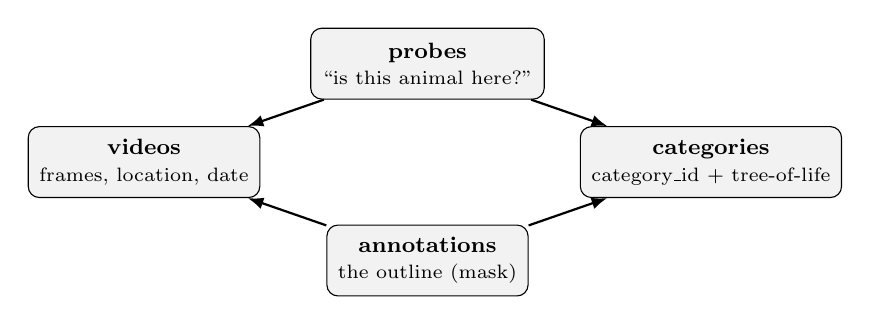
\begin{tikzpicture}
  \node[data] (vid) at (0,0) {\textbf{videos}\\{\scriptsize frames, location, date}};
  \node[data] (cat) at (7.2,0) {\textbf{categories}\\{\scriptsize category\_id $+$ tree-of-life}};
  \node[data] (pair) at (3.6,1.25) {\textbf{probes}\\{\scriptsize ``is this animal here?''}};
  \node[data] (ann) at (3.6,-1.25) {\textbf{annotations}\\{\scriptsize the outline (mask)}};
  \draw[flow] (pair) -- (vid); \draw[flow] (pair) -- (cat);
  \draw[flow] (ann) -- (vid);  \draw[flow] (ann) -- (cat);
\end{tikzpicture}
\caption{How SA-FARI is wired together, and what \code{records()} untangles. A \emph{probe} asks whether a
named animal (a \code{category\_id}) appears in a video; \emph{annotations} give the ground-truth outlines
for the ones that do. The identity is the \code{category\_id}, not the prompt text --- two prompts can mean
the same species --- so everything keys on it.}
\label{fig:schema}
\end{figure}

\takeaway{Every raw (video, prompt) probe becomes one typed \code{VideoRecord} with its species resolved
from \code{category\_id} and absent-species probes flagged as hard negatives --- a clean, trusted unit for
the whole pipeline.}

% =====================================================================
\section{Step 2 --- The two experiments (and the leakage firewall)}

\paragraph{The point.}
The whole idea rests on a \emph{reference} (``what we've seen'') and a \emph{probe} (``the new thing''): a
distance measures how far a probe sits from the reference. Inspecting the data changed the plan here. The
official split holds out \emph{new places} but re-uses the \emph{same species} on both sides --- so on that
split ``species novelty'' is always zero. Because SAM\,3 is \textbf{frozen} (it never trains on any of
this), the split is only \emph{our} choice of reference, and we are free to re-slice it. So we run
\textbf{two complementary experiments} (Fig.~\ref{fig:splits}): a \textbf{species hold-out}
(leave-one-species-out --- the detection/novelty test, H1) and the official \textbf{location hold-out} (the
environment/association test, H2). A leakage firewall then guarantees that the axis under test is genuinely
disjoint, so a later ``prediction'' can never be explained by the model having already seen the answer.

\srcfile{src/splits.py}
\begin{lstlisting}[style=py]
def build_species_partition(config: Config | None = None) -> Partition:
    """Split A — leave-one-species-out over the pooled present set."""
    cfg = config or Config()
    records = _present(pooled_records(cfg))
    species = sorted({r.category_id for r in records})
    locations = _locations(records)
    return Partition(
        name="species_holdout",
        held_axis="species",
        loso=True,
        reference_species=species,
        probe_species=species,
        reference_locations=locations,
        probe_locations=locations,
        reference_years=_years(records),
        probe_origins=["train", "test"],
    )
\end{lstlisting}

\paragraph{In the code.}
\code{build\_species\_partition} constructs Split A, the primary species hold-out. First
\code{\_present(pooled\_records(cfg))} pools the train and test videos together and keeps only records that
actually contain an animal (\code{r.num\_masklets > 0}) --- the positive probes. It then collects the
distinct species (\code{category\_id}) and the real location ids into sorted lists. Crucially,
\code{reference\_species} and \code{probe\_species} are set to the \emph{same} full list, and likewise for
locations: every species is both a probe \emph{and} part of the reference pool. The disjointness that makes
this a fair test is \emph{not} done by deleting species here --- it is deferred, signalled by
\code{loso=True} (leave-one-species-out). The idea: when we later measure how novel a given species is, we
compute its distance to all the \emph{other} reference species, excluding itself, so a species is never
judged similar to itself. \code{held\_axis="species"} records the axis under test, and
\code{probe\_origins=["train", "test"]} says probes may come from either source file (pooling ignores the
official split for this experiment). The result is a small, frozen Pydantic record describing the whole
experiment, saved to JSON so every downstream distance is computed against exactly this fixed anchor.

\begin{figure}[h]
\centering
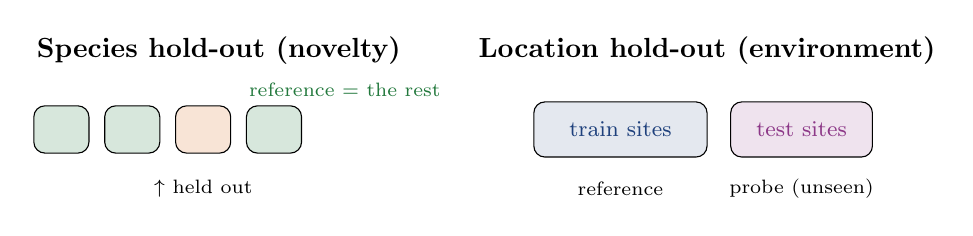
\begin{tikzpicture}[font=\footnotesize]
  % species hold-out
  \begin{scope}
    \node[font=\bfseries] at (2,1.4) {Species hold-out (novelty)};
    \foreach \x/\c in {0/forest,1/forest,2/burnt,3/forest} {
      \node[draw,rounded corners,fill=\c!18,minimum width=7mm,minimum height=6mm] at (\x*0.9,0.4) {};}
    \node[font=\scriptsize] at (2*0.9,-0.35) {$\uparrow$ held out};
    \node[forest,font=\scriptsize] at (3.6,0.9) {reference $=$ the rest};
  \end{scope}
  % location hold-out
  \begin{scope}[xshift=6.2cm]
    \node[font=\bfseries] at (2,1.4) {Location hold-out (environment)};
    \draw[rounded corners,fill=navy!12] (-0.2,0.05) rectangle (2.0,0.75);
    \node[navy] at (0.9,0.4) {train sites};
    \draw[rounded corners,fill=plum!14] (2.3,0.05) rectangle (4.1,0.75);
    \node[plum] at (3.2,0.4) {test sites};
    \node[font=\scriptsize] at (0.9,-0.35) {reference};
    \node[font=\scriptsize] at (3.2,-0.35) {probe (unseen)};
  \end{scope}
\end{tikzpicture}
\caption{Two ways to slice the same data. \textbf{Left}: each species is held out in turn and compared to
the others (species varies, place stays familiar). \textbf{Right}: the official geographic split (place
varies, species stays familiar). Together they isolate the two hypotheses.}
\label{fig:splits}
\end{figure}

\takeaway{Split A defines the species-novelty experiment as one frozen reference/probe record, deferring
true disjointness to a per-species leave-one-out step (\code{loso=True}) instead of physically removing
species --- and a test (Step 6) proves that firewall actually holds.}

% =====================================================================
\section{Step 3 --- The four ``how new is it?'' distances}
Each distance answers a plain question and is computed with \emph{no label of the target animal}. Two of
them (taxonomic, temporal) are pure lookups; two (visual, environment) share one embedding engine.

\subsection*{Taxonomic --- how far apart on the tree of life?}

\paragraph{The point.}
Every test species needs a single number for ``how unfamiliar is this animal, taxonomically, versus what the
model has seen?'' We answer it by measuring how far the species sits from the \emph{nearest} training-set
species on the biological tree of life, Kingdom\,$\to$\,Species (Fig.~\ref{fig:tree}). It is label-free ---
it uses only each species' taxonomy path, never any tracking result --- so it can be computed \emph{before}
running the tracker. The self-exclusion (LOSO) rule stops a species ever counting itself as its own
neighbour, which would trivially make everything look familiar (distance $0$) and leak information.

\srcfile{src/features/taxonomic.py}
\begin{lstlisting}[style=py]
def tree_distance(a: list[str], b: list[str]) -> int:
    # same genus -> 1, same family -> 2, same order -> 3, fully disjoint -> 7
    shared = 0
    for x, y in zip(a, b, strict=False):
        if x and x == y:
            shared += 1
        else:
            break
    return len(a) - shared

# ... in TaxonomicDistance.compute:
    for cid in partition.probe_species:
        if cid not in paths:
            rows[cid] = float("nan")
            continue
        others = [paths[c] for c in reference if not (partition.loso and c == cid)]
        rows[cid] = (
            float(min(tree_distance(paths[cid], p) for p in others)) if others else float("nan")
        )
\end{lstlisting}

\paragraph{In the code.}
\code{tree\_distance} takes two taxonomy paths, each an ordered list of names from Kingdom down to Species.
It walks them level by level in lockstep: while the names match and are non-empty it counts shared ancestry
(\code{shared += 1}); the moment they differ or a level is blank it stops. The answer is
\code{len(a) - shared}, i.e.\ how many levels you must climb to reach the lowest common ancestor. So two
species in the same genus differ only at the last level and score $1$; sharing only the family scores $2$;
the order, $3$; and two fully unrelated 7-level paths score $7$. In \code{compute}, for each probe species
\code{cid} it first checks the species has a full path (else record \code{NaN} and skip). It then builds
\code{others}: the reference species' paths, but with the LOSO guard
\code{not (partition.loso and c == cid)} dropping the probe species itself whenever the split is
leave-one-species-out. Finally it takes \code{tree\_distance} to every remaining reference species and keeps
the \emph{minimum} --- the distance to the nearest known relative --- falling back to \code{NaN} if
self-exclusion emptied the reference.

\begin{figure}[h]
\centering
\begin{minipage}[c]{0.44\textwidth}\centering
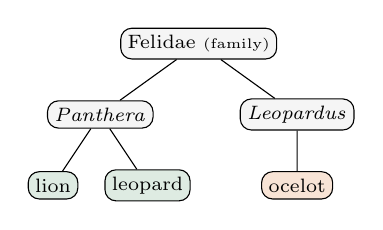
\begin{tikzpicture}[font=\scriptsize,
   level 1/.style={sibling distance=25mm,level distance=9mm},
   level 2/.style={sibling distance=12mm,level distance=9mm},
   every node/.style={draw,rounded corners,inner sep=2.5pt,fill=black!4}]
  \node {Felidae {\tiny(family)}}
    child {node {\emph{Panthera}}
      child {node[fill=forest!15] {lion}}
      child {node[fill=forest!15] {leopard}}}
    child {node {\emph{Leopardus}}
      child {node[fill=burnt!18] {ocelot}}};
\end{tikzpicture}
\captionof{figure}{Lion\,$\leftrightarrow$\,leopard share a genus (distance $1$); lion\,$\leftrightarrow$\,
ocelot share only the family (distance $2$).}
\label{fig:tree}
\end{minipage}\hfill
\begin{minipage}[c]{0.52\textwidth}\centering
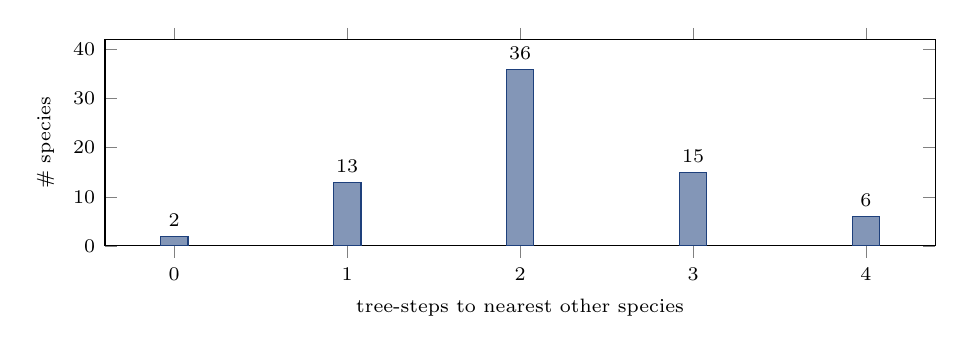
\begin{tikzpicture}
\begin{axis}[width=\textwidth,height=4.2cm,ybar,bar width=10pt,
  xlabel={tree-steps to nearest other species},ylabel={\# species},
  xtick={0,1,2,3,4},ymin=0,ymax=42,nodes near coords,
  every node near coord/.append style={font=\scriptsize},
  tick label style={font=\scriptsize},label style={font=\scriptsize}]
\addplot[fill=navy!55,draw=navy] coordinates {(0,2)(1,13)(2,36)(3,15)(4,6)};
\end{axis}
\end{tikzpicture}
\captionof{figure}{Measured leave-one-species-out distances (72 species). Real numbers from our run: most
animals have a same-family neighbour, but a fifth are clearly novel ($\ge 3$). The two $0$s are a quirk ---
``pig'' and ``wild boar'' are the same species under two names.}
\label{fig:taxhist}
\end{minipage}
\end{figure}

\takeaway{One label-free number per test species: tree steps to its nearest training relative, with
self-exclusion so a species can never be its own neighbour. Across 72 species the spread runs $0$--$4$
(Fig.~\ref{fig:taxhist}) --- enough variation to make the novelty axis testable.}

\subsection*{Temporal --- how many years apart?}
The simplest one, and a pure lookup like the taxonomic distance: the number of years between the probe's
footage and the nearest reference footage (SA-FARI spans 2014\,$\rule[0.4ex]{5mm}{0.6pt}$\,2024). A 2023
clip against a 2015 reference is a gap of $8$. It guards against confusing ``old camera hardware'' with
``novel animal''.

\subsection*{Visual + environment --- how unfamiliar does it \emph{look}?}

\paragraph{The point.}
The visual and environment distances work the same way: turn each animal (or scene) into a fixed-length
``fingerprint'' vector from a frozen vision encoder, average those into one \textbf{prototype} per species
(or per site), and measure how far a probe sits from the nearest \emph{other} prototype. Rather than
duplicate this in two feature modules, the shared logic lives in one place (\code{pipeline.py}) so each
feature only supplies the two things that actually differ: \emph{which crop} to embed and \emph{what to
group by}. The distance is deliberately a simple, bounded ``$1$ minus cosine similarity'' so it feeds
cleanly into the downstream predictor without ever peeking at a target's label.

\srcfile{src/features/pipeline.py}
\begin{lstlisting}[style=py]
def prototype(vectors: list[np.ndarray]) -> np.ndarray | None:
    """Re-normalised mean of L2-normalised vectors (``None`` if there are none)."""
    if not vectors:
        return None
    mean = np.mean(vectors, axis=0)
    return mean / max(float(np.linalg.norm(mean)), 1e-12)


def nearest_distance(
    vector: np.ndarray, references: dict[str, np.ndarray], exclude: str | None = None
) -> float:
    """``1 - max cosine`` to the nearest reference prototype (skipping ``exclude``); ``NaN`` if none."""
    candidates = [proto for key, proto in references.items() if key != exclude]
    if not candidates:
        return float("nan")
    return 1.0 - max(float(vector @ proto) for proto in candidates)
\end{lstlisting}

\paragraph{In the code.}
\code{prototype} takes a list of per-crop embedding vectors (each already unit-length from the encoder) and
collapses them into a single representative direction: it averages them element-wise, then re-normalises so
the result is again a unit vector pointing at that group's ``average look''. It returns \code{None} when a
group produced no usable crops, which is how a \code{NaN} distance later surfaces honestly.
\code{nearest\_distance} then compares one probe vector against a dictionary of reference prototypes. Because
all vectors are unit-length, the dot product \code{vector @ proto} \emph{is} the cosine similarity ($1.0$
identical, $0$ unrelated). It takes the \emph{maximum} similarity over all references --- the single closest
neighbour --- and reports $1 - \text{that}$, so a small number means ``looks familiar, close to something
seen'' and a larger number means ``novel''. The \code{exclude} argument is the leave-one-out guard: on the
species split a probe's own prototype is also in the reference set, so it is skipped by key to stop a species
matching itself and scoring $0$. The \code{embed\_crops} engine (same file) feeds these two functions: it is
cache-first (only cache-miss crops trigger work), batch-fetches the missing frames per video, embeds once,
writes back to the cache, and returns \code{\{key: vector\}} --- the raw material \code{prototype} averages.
The \textbf{environment} distance is the very same picture with the animal \emph{erased} (its pixels filled
with the average background) instead of cut out, grouped by location instead of species, plus a night/IR
flag that fires when a frame is basically grey.

\begin{figure}[h]
\centering
\begin{minipage}[c]{0.60\textwidth}\centering
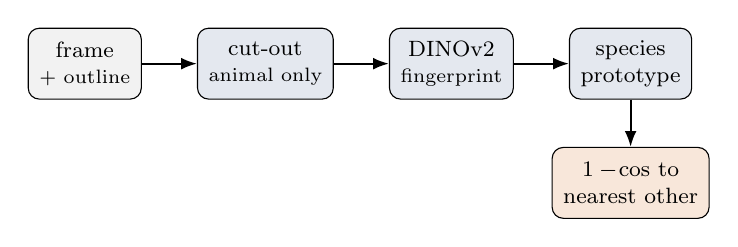
\begin{tikzpicture}[node distance=4mm and 7mm]
  \node[data] (fr) {frame\\{\scriptsize $+$ outline}};
  \node[work,right=of fr] (crop) {cut-out\\{\scriptsize animal only}};
  \node[work,right=of crop] (emb) {DINOv2\\{\scriptsize fingerprint}};
  \node[work,right=of emb] (proto) {species\\prototype};
  \node[resbox,below=6mm of proto] (dist) {$1-\!\cos$ to\\nearest other};
  \draw[flow] (fr)--(crop); \draw[flow] (crop)--(emb); \draw[flow] (emb)--(proto);
  \draw[flow] (proto)--(dist);
\end{tikzpicture}
\captionof{figure}{The visual distance, end to end --- the pipeline \code{embed\_crops}\,$\to$\,
\code{prototype}\,$\to$\,\code{nearest\_distance} draws. ``Environment'' is the same picture with the animal
\emph{erased} instead of cut out, grouped by location.}
\label{fig:vispipe}
\end{minipage}\hfill
\begin{minipage}[c]{0.36\textwidth}\centering
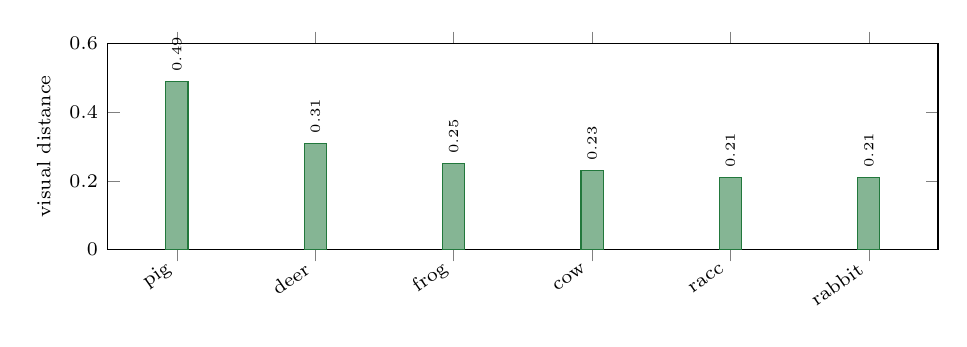
\begin{tikzpicture}
\begin{axis}[width=\textwidth,height=4.2cm,ybar,bar width=8pt,
  symbolic x coords={pig,deer,frog,cow,racc,rabbit},xtick=data,
  x tick label style={rotate=35,anchor=east,font=\scriptsize},
  ylabel={visual distance},ymin=0,ymax=0.6,nodes near coords,
  every node near coord/.append style={font=\tiny,rotate=90,anchor=west},
  tick label style={font=\scriptsize},label style={font=\scriptsize}]
\addplot[fill=forest!55,draw=forest] coordinates
  {(pig,0.49)(deer,0.31)(frog,0.25)(cow,0.23)(racc,0.21)(rabbit,0.21)};
\end{axis}
\end{tikzpicture}
\captionof{figure}{Measured visual distances (six-species subset). Real numbers: the pig looks most
distinct, the smaller mammals cluster together.}
\label{fig:visbar}
\end{minipage}
\end{figure}

\takeaway{One tiny, shared, label-free engine --- embed once, average into prototypes, take $1$ minus
nearest cosine --- powers both the visual and environment distances, with a leave-one-out guard so nothing
matches itself. On the location hold-out the environment distances ran $\approx 0.06$--$0.44$, with the
infrared night sites flagged correctly and the daytime colour sites not.}

% =====================================================================
\section{Step 4a --- Measuring SAM\,3 (the inference harness)}

\paragraph{The point.}
This is where we actually run the frozen tracker on every test clip and record what it found. \textbf{SAM\,3}
is a \emph{promptable} tracker: give it a text prompt (``ocelot'') and it finds and follows every matching
animal across the video, with no training on that species. The step has to survive real-world
interruptions: the model runs on a borrowed Colab GPU that times out mid-job, and the test split has
thousands of clips. So the harness is \textbf{restartable} --- it writes one small results file per video
and never redoes a video it has already done. A run that dies after 400 clips picks up at clip 401 instead
of starting over. Separately, the tracker is loaded only when first needed, so all the analysis code (and
the tests) can import this module on a plain laptop with no GPU.

\srcfile{src/inference/harness.py}
\begin{lstlisting}[style=py]
def run(self, split: str = "test", limit: int | None = None) -> Path:
    """Predict masklets for every probe and write per-video JSONs; return the predictions dir."""
    out_dir = self._out_dir(split)
    out_dir.mkdir(parents=True, exist_ok=True)
    records = SAFARI(split, self.config).records()
    if limit is not None:
        records = records[:limit]

    for i, record in enumerate(records):
        path = out_dir / f"{record.video_id}.json"
        if path.exists():
            continue  # resumable: already predicted
        path.write_text(json.dumps(self._predict_video(record)))
        if (i + 1) % 50 == 0:
            print(f"  {i + 1}/{len(records)} probes predicted")

    combined = [json.loads(p.read_text()) for p in sorted(out_dir.glob("*.json"))]
    combined_path = out_dir.with_suffix(".json")
    combined_path.write_text(json.dumps({"predictions": combined}))
    print(f"predictions -> {out_dir} ({len(combined)} videos) | combined -> {combined_path}")
    return out_dir
\end{lstlisting}

\paragraph{In the code.}
Top to bottom: \textbf{(1)} \code{\_out\_dir(split)} picks an output folder keyed by \emph{both} the split
and the prompt mode (species-specific vs.\ the generic ``animal'' run), so the two experimental conditions
never overwrite each other. \textbf{(2)} \code{SAFARI(split).records()} loads the list of every clip to
run; \code{limit} optionally trims it to a handful for a quick smoke test. \textbf{(3)} the loop is the
heart of it: for each clip it computes the output path \code{<video\_id>.json}, and if that file already
exists it does \code{continue} --- that single \code{if path.exists(): continue} is what makes the whole job
resumable after a Colab timeout. \textbf{(4)} otherwise it calls \code{\_predict\_video(record)}, which loads
the frames and calls \code{self.tracker.track(frames, prompt)} to run SAM\,3, then writes the result
straight to disk as JSON --- so progress is saved one video at a time, not buffered in memory. \textbf{(5)}
a progress line prints every 50 clips. \textbf{(6)} after the loop it re-reads all the per-video JSONs
(sorted for a stable order) and concatenates them into one combined \code{predictions.json} that the
official evaluator consumes. The per-video files are the durable source of truth; the combined file is just
rebuilt from them each time, so it is always consistent with whatever has finished.

\begin{figure}[h]
\centering
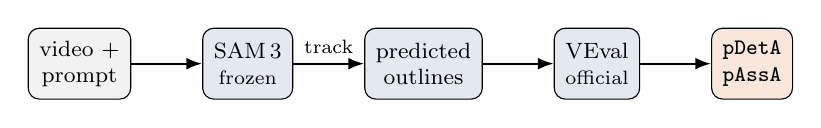
\begin{tikzpicture}[node distance=4mm and 9mm]
  \node[data] (v) {video $+$\\prompt};
  \node[work,right=of v] (s) {SAM\,3\\{\scriptsize frozen}};
  \node[work,right=of s] (m) {predicted\\outlines};
  \node[work,right=of m] (ve) {VEval\\{\scriptsize official}};
  \node[resbox,right=of ve] (sc) {\code{pDetA}\\\code{pAssA}};
  \draw[flow] (v)--(s); \draw[flow] (s)--node[midway,above,font=\scriptsize]{track}(m);
  \draw[flow] (m)--(ve); \draw[flow] (ve)--(sc);
\end{tikzpicture}
\caption{Measuring the ground truth. A prompt goes into frozen SAM\,3, which outlines and tracks matches;
the official scorer turns that into \code{pDetA} (\emph{did it find the animals?}) and \code{pAssA}
(\emph{did it keep each identity over time?}). We analyse the two separately --- that is the intellectual
core of the project.}
\label{fig:meas}
\end{figure}

\takeaway{A crash-proof, restartable measurement run: one JSON per video plus skip-if-exists means a
timed-out GPU job resumes instead of restarting, and the model only loads when actually tracking. Built and
tested with a stand-in; the real run happens on a GPU.}

% =====================================================================
\section{Step 4b --- Scoring to per-cell \code{pDetA} / \code{pAssA}}

\paragraph{The point.}
The official VEval evaluator scores each individual (video, prompt) probe, but the dissertation's unit of
analysis is the \emph{cell} --- a (species, location, year) group. This step is the funnel that turns many
raw per-probe metrics into one clean row per cell, while also counting how much annotated data stands behind
each score. That support count matters: a cell backed by 3 labelled frames should not be trusted like one
backed by 300, so the later regression \emph{weights} by it and \emph{controls} for it --- that is how
``rare'' is never confused with ``far'' (novel).

\srcfile{src/eval/score.py}
\begin{lstlisting}[style=py]
def aggregate(self, per_probe: dict[tuple[str, str], dict], split: str) -> pd.DataFrame:
    safari = SAFARI(split, self.config)
    support = self._support(split)
    cells: dict[tuple, dict] = defaultdict(
        lambda: {m: [] for m in _METRICS} | {"n_frames": 0, "n_masklets": 0, "n_videos": 0}
    )
    for record in safari.records():
        cell = safari.cell_of(record)
        agg = cells[(cell.category_id, cell.species, cell.location_id, cell.time)]
        metrics = per_probe.get((record.video_id, record.category_id))
        if metrics:
            for m in _METRICS:
                if metrics.get(m) is not None:
                    agg[m].append(float(metrics[m]))
        n_frames, n_masklets = support.get((record.video_id, record.category_id), (0, 0))
        agg["n_frames"] += n_frames
        agg["n_masklets"] += n_masklets
        agg["n_videos"] += 1
    # ... build one row per cell ...
    **{m: float(np.mean(agg[m])) if agg[m] else float("nan") for m in _METRICS},
\end{lstlisting}

\paragraph{In the code.}
First it asks the dataset for the support table (via \code{\_support}) --- a lookup from each probe to how
many labelled frames and masklets back it. It then creates \code{cells}, a dictionary that auto-initialises
any new cell with empty metric lists and zero counters. It walks every probe \code{record};
\code{safari.cell\_of(record)} collapses that probe down to its cell key --- the four coordinates
(\code{category\_id}, \code{species}, \code{location\_id}, and the year from the timestamp) --- so every
video of the same species at the same place in the same year lands in the same bucket. It looks up that
probe's VEval metrics by the \code{(video\_id, category\_id)} key; if present, each of
\code{pDetA}/\code{pAssA}/\code{pHOTA} that is not \code{None} is appended to the cell's running list.
Regardless of whether metrics exist, it adds this probe's frame and masklet counts to the cell's totals and
bumps the video count. After the loop each cell becomes one output row: the three metrics are collapsed to a
plain mean over the probes in that cell (or \code{NaN} if none produced that metric), and the support
counters and prompt condition are attached. The result is a tidy DataFrame with exactly one row per cell ---
the dependent variables the later analysis fits its ``law'' against.

\takeaway{Collapses many per-probe VEval scores into one row per (species, location, year) cell --- the
analysis unit --- each carrying its own support counts so scores can be trust-weighted and ``rare'' is
never mistaken for ``far''.}

% =====================================================================
\section{Step 5 --- Fitting the law (planned)}
With the distances ($X$) and scores ($Y$) in hand, the last stage fits a small, honest model:
\begin{itemize}
  \item \textbf{A curve, not a black box.} A beta regression (a straight line through a ``squashing''
        transform, because scores live in $[0,1]$) maps distances to a predicted score --- one model for
        detection, one for association, each weighted by support.
  \item \textbf{Which factor matters?} Variance partitioning asks whether \emph{detection} is driven by
        \emph{species novelty} and \emph{association} by \emph{environment} --- the headline contrast.
  \item \textbf{Does it generalise?} We hide whole species (and whole places), predict them from distance
        \emph{alone}, and check the prediction lands near the truth, with honest error bars
        (Fig.~\ref{fig:predline}). Success is a \emph{validated} predictor, not a higher score.
  \item \textbf{The tool.} Four distances in $\to$ predicted \code{pDetA}/\code{pAssA} $+$ a confidence
        interval out: the practical ``will it work here?'' answer.
\end{itemize}

\begin{figure}[h]
\centering
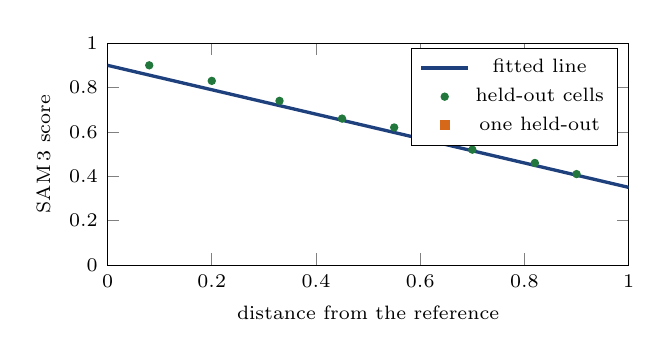
\begin{tikzpicture}
\begin{axis}[width=8.2cm,height=4.4cm,
  xlabel={distance from the reference},ylabel={SAM\,3 score},
  xmin=0,xmax=1,ymin=0,ymax=1,tick label style={font=\scriptsize},label style={font=\scriptsize},
  legend style={font=\scriptsize,at={(0.98,0.98)},anchor=north east}]
  \addplot[navy,very thick,domain=0:1]{0.9-0.55*x};
  \addplot[only marks,mark=*,mark size=1.3pt,forest]
    coordinates {(0.08,0.9)(0.2,0.83)(0.33,0.74)(0.45,0.66)(0.55,0.62)(0.7,0.52)(0.82,0.46)(0.9,0.41)};
  \addplot[burnt,mark=square*,mark size=1.6pt,only marks] coordinates {(0.6,0.58)};
  \legend{fitted line, held-out cells, one held-out}
\end{axis}
\end{tikzpicture}
\caption{The target picture (\emph{illustrative --- pending the real scores}): predict a held-out cell's
score from its distance and check it lands on the line, with bootstrap confidence intervals.}
\label{fig:predline}
\end{figure}

% =====================================================================
\section{Step 6 --- The rule that keeps it honest (config $+$ tests)}

\paragraph{The point.}
The whole project hinges on one rule: \emph{no test-set information may leak into a ``before you run it''
prediction}, or the predictor becomes trivially perfect and the science is worthless. Two pillars enforce
it. First, a single Pydantic-settings \code{Config} holds every constant (paths, dataset facts, inference,
scoring, distances, model, cross-validation), so experiments change a \emph{value}, never the code, and any
field can be overridden by a \code{SAFARI\_*} environment variable or a YAML file. Second, the tests turn
the hard rules into checks that fail loudly. The one below proves that when we measure how ``far'' an
unseen species is, the species is \emph{never} compared against itself (which would fake a distance of
zero).

\srcfile{tests/test\_leakage.py}
\begin{lstlisting}[style=py]
@_needs_ann
def test_loso_excludes_self() -> None:
    """Leave-one-species-out never lets a species be its own reference (else every distance is 0)."""
    part = build_species_partition(_CFG)
    loso = TaxonomicDistance(_CFG).compute(part).dropna()
    with_self = TaxonomicDistance(_CFG).compute(part.model_copy(update={"loso": False})).dropna()

    assert (with_self == 0).all()  # self-inclusion collapses every distance to 0
    assert (loso > 0).sum() > 0    # LOSO recovers the real (mostly non-zero) distances
    assert not loso.equals(with_self)
\end{lstlisting}

\paragraph{In the code.}
This is the leave-one-species-out leakage guard, and it tests exactly the firewall from Step 2. If a species
were ever allowed into its own reference set, its nearest reference would be itself, so the distance would
collapse to zero --- a fake, leaked answer. The test builds the species partition, then computes the
distance two ways. \code{loso} is the correct mode: each species excluded from its own comparison set.
\code{with\_self} deliberately turns that protection off (\code{model\_copy(update=\{"loso": False\})}), a
clean, immutable way to flip one setting on the Pydantic partition without mutating the original. The three
assertions pin the behaviour down: with self-inclusion \emph{every} distance is exactly $0$ (leakage
confirmed present when protection is off), with LOSO many distances are strictly positive (real structure
recovered), and the two disagree. If someone ever broke the exclusion, the middle assertion would fail and
the build would go red. The \code{\_needs\_ann} marker skips the test cleanly when the gated annotations are
not downloaded, so the suite stays green on a fresh checkout.

\takeaway{A red-if-broken guard that the central ``no test-set leakage'' rule actually holds --- a species
can never fake a zero distance by anchoring on itself --- backed by a config that makes every experiment a
value change, not a code change.}

% =====================================================================
\section{Where we are, and the next step}
The \textbf{distance side is finished and sanity-checked} on real data, and the \textbf{measurement side is
built}. The codebase is typed, configuration-driven, lint-clean, and covered by a growing test suite; the
label-free features were refactored and verified to reproduce their outputs exactly. The immediate milestone
is the \textbf{first decision gate}: run frozen SAM\,3 over the test split on Colab (weights access is
confirmed), score it with VEval, aggregate to cells, and check the numbers sit in SA-FARI's published SAM\,3
range. Passing that gate opens the modelling half --- fitting the detection-versus-association law and
building the reliability estimator.

\end{document}
